\subsection{Server}

L'architettura della componente server si articola in una 3-layer architecture, in cui si identificano i seguenti layer:
\begin{itemize}
	\item \textbf{Communication layer}
	\item \textbf{Business layer}
	\item \textbf{Persistence layer}
\end{itemize}

\begin{figure}[H]
	\centering
	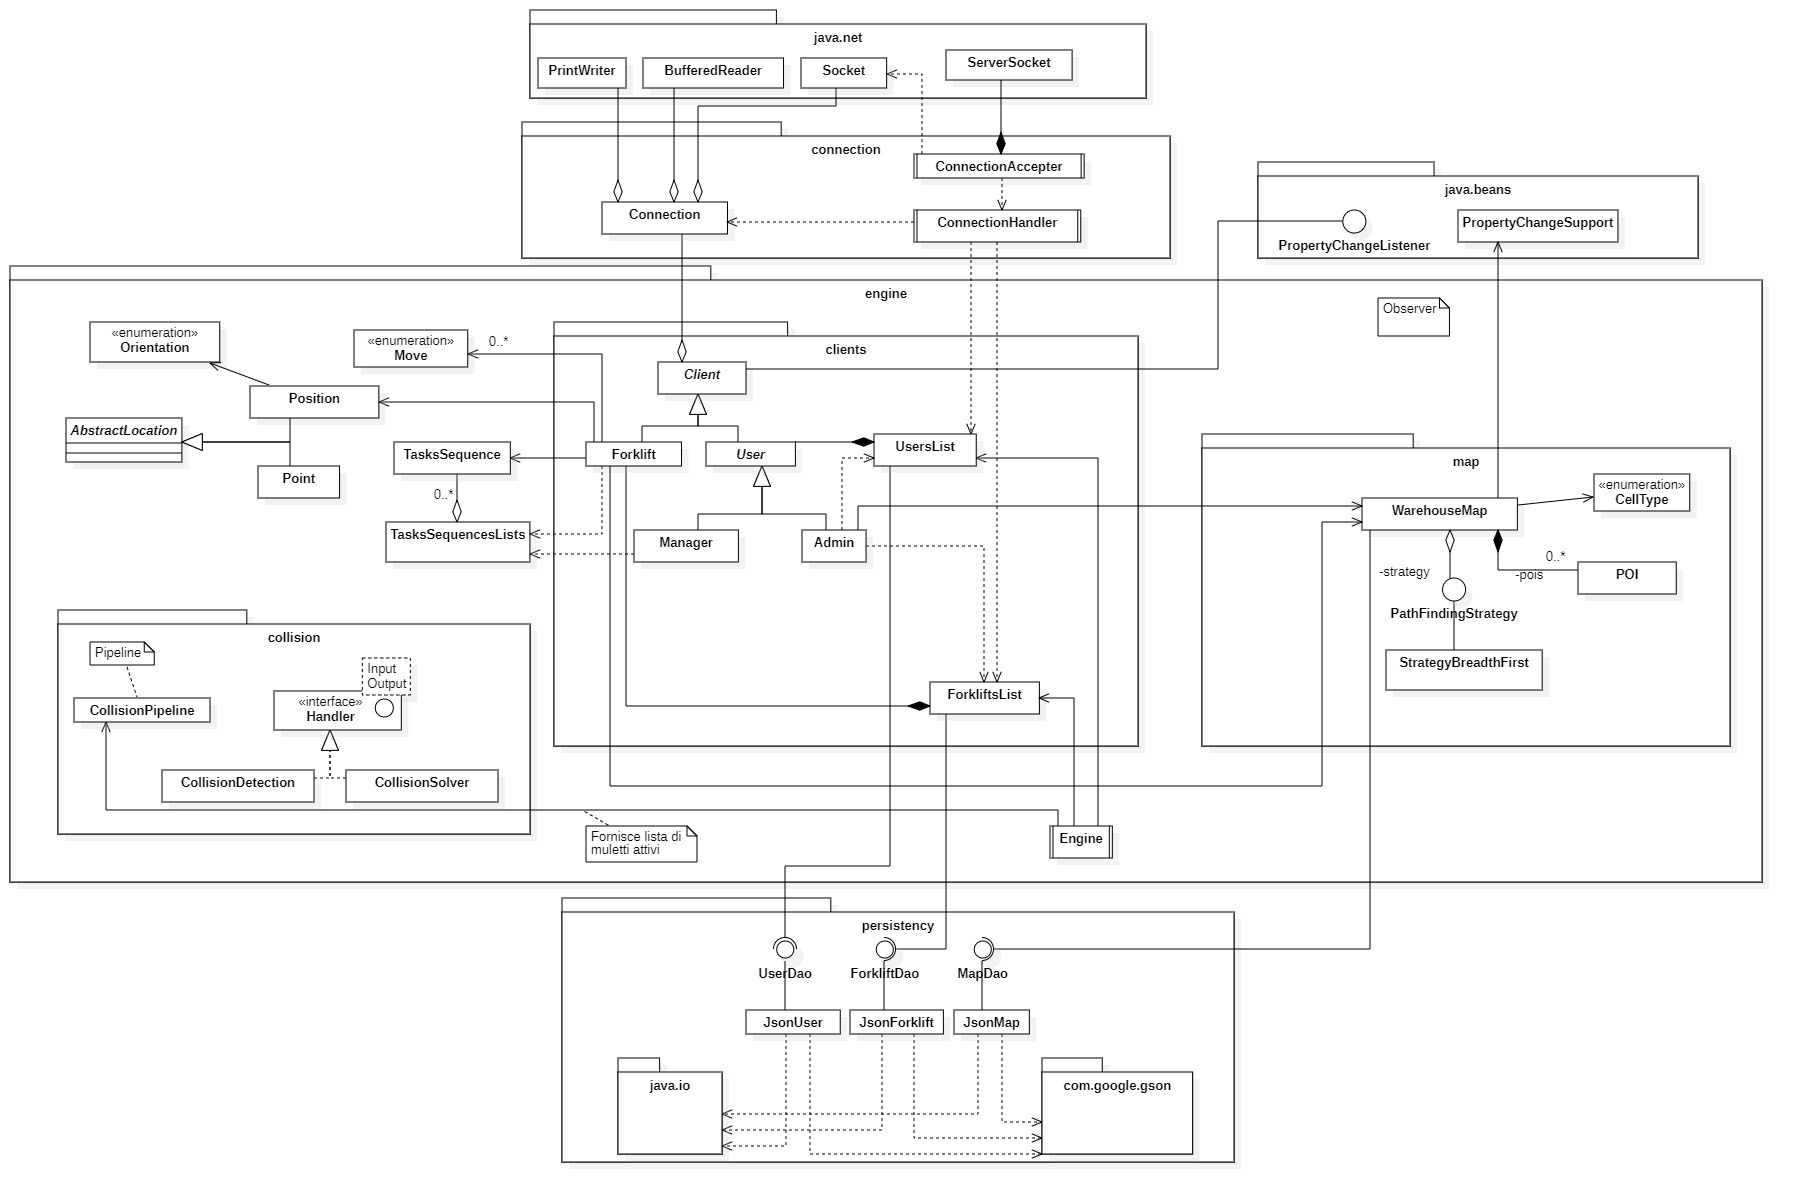
\includegraphics[scale=0.22]{res/diagrams/server/server_complessivo_minimal.jpg}
	\caption{Visione complessiva dell'architettura del server}
\end{figure}

Le sezioni che seguono illustrano la struttura di ogni layer.

\subsubsection{Communication layer}

\begin{figure}[H]
	\centering
	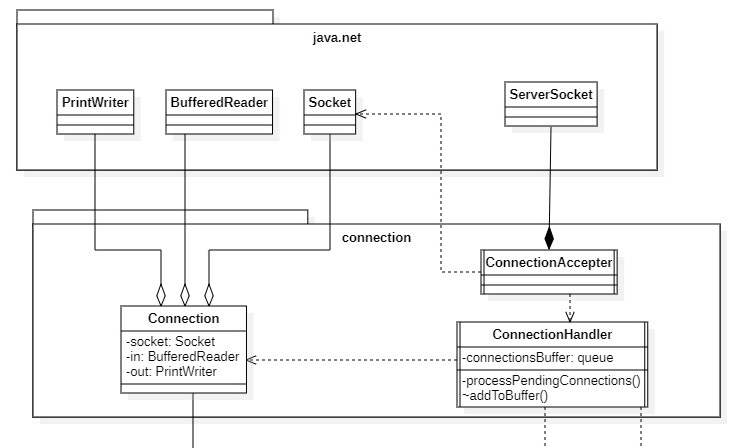
\includegraphics[scale=0.55]{res/diagrams/server/server_communication.jpg}
	\caption{Visione di dettaglio del Communication Layer}
\end{figure}


\subsubsection{Business layer}

\begin{figure}[H]
	\centering
	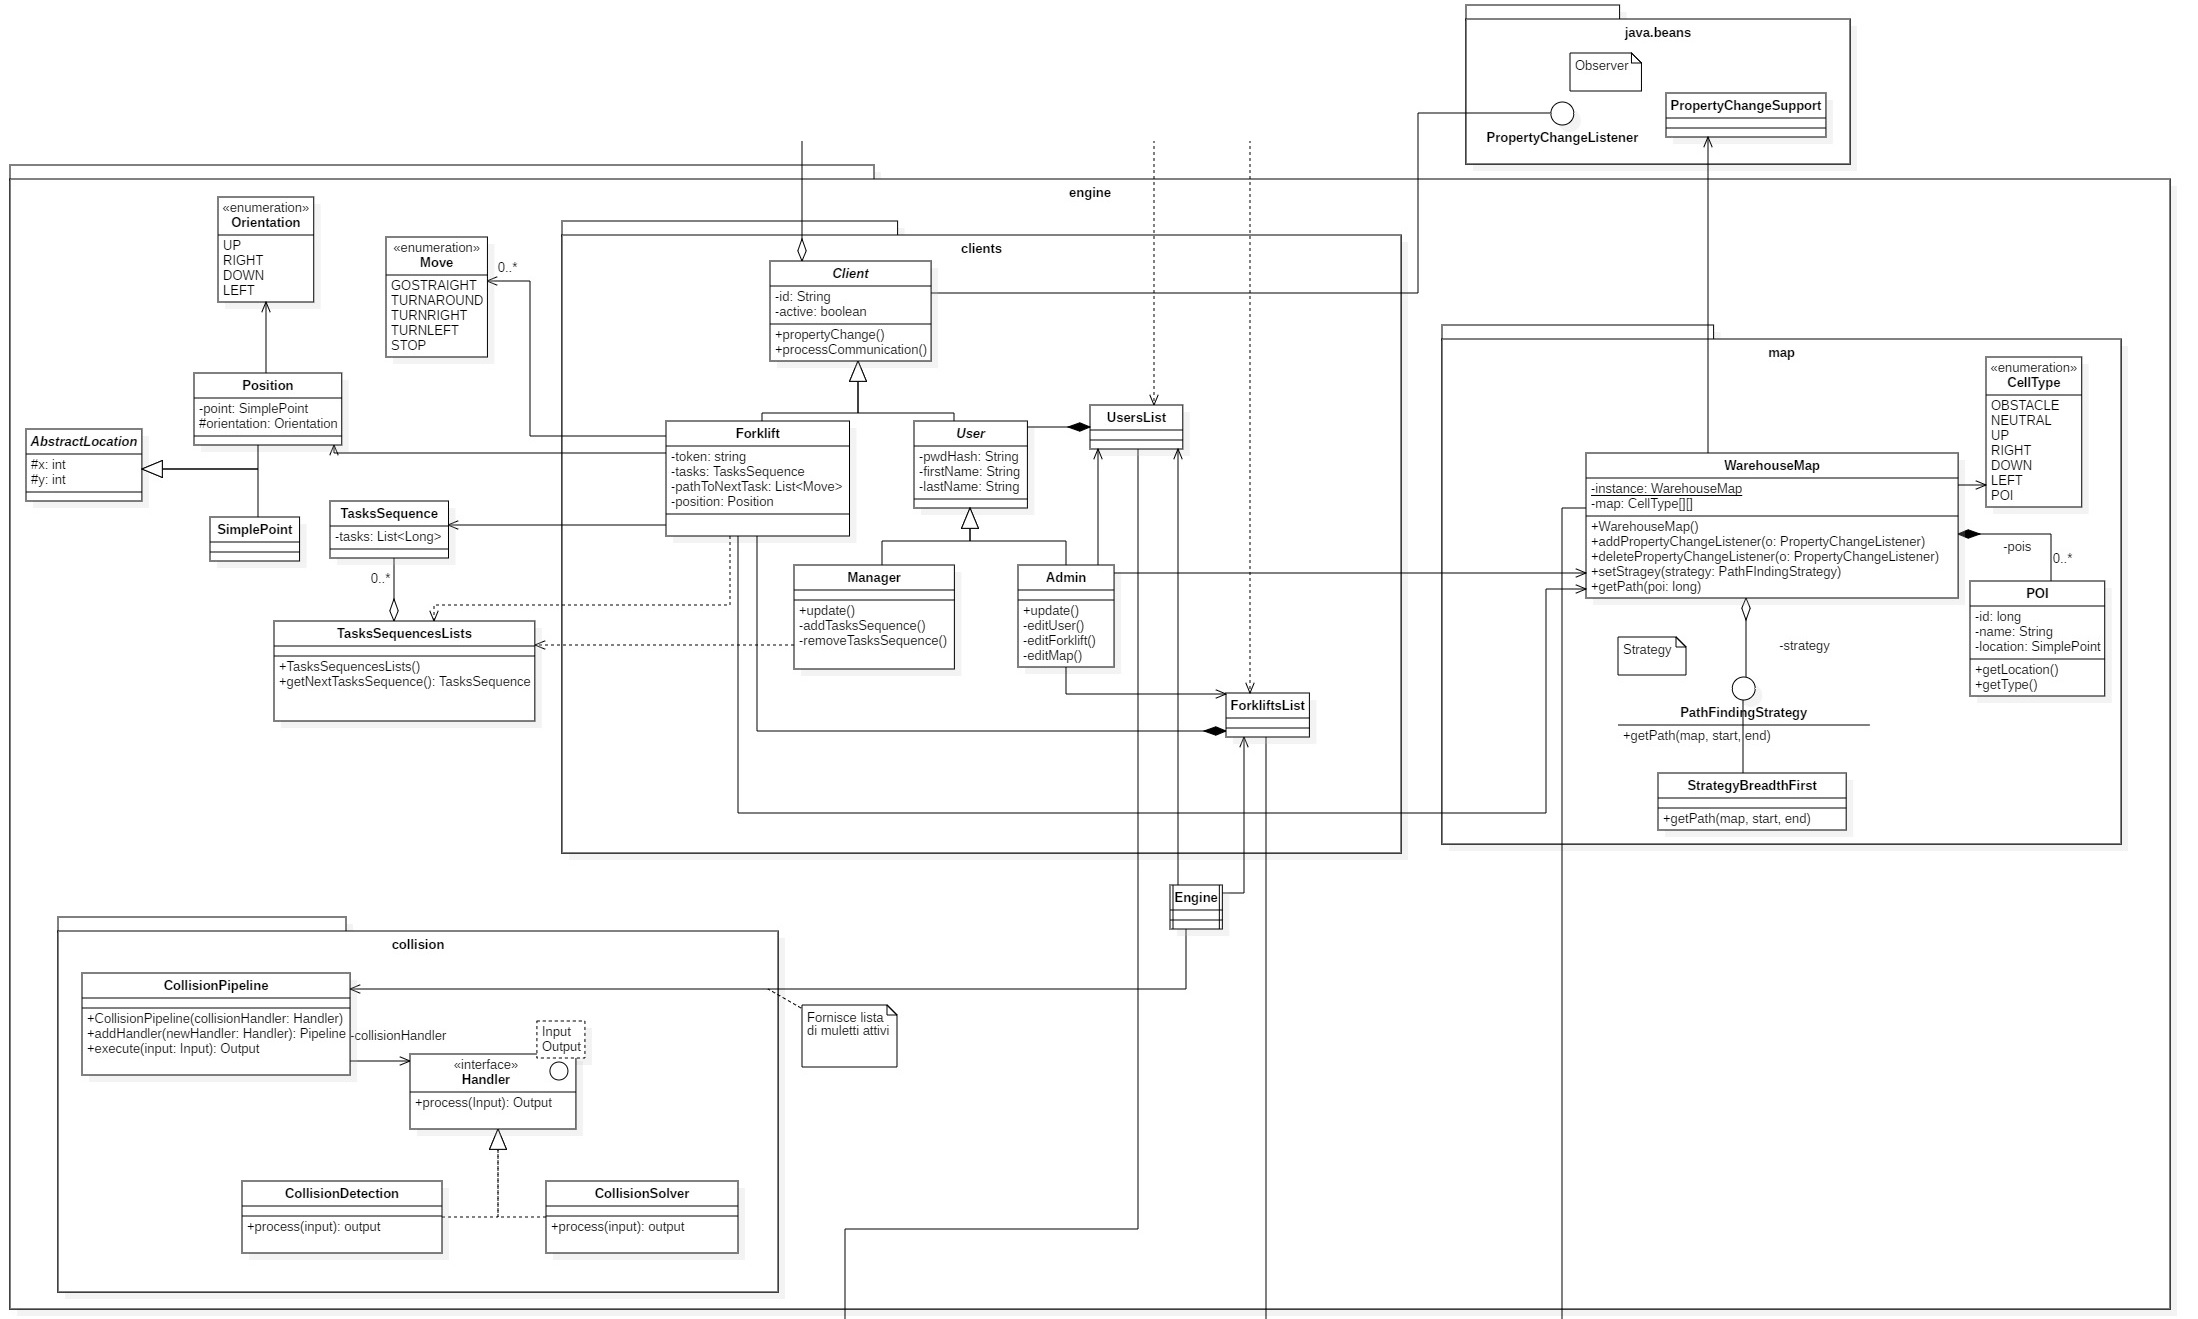
\includegraphics[scale=0.26]{res/diagrams/server/server_business.jpg}
	\caption{Visione di dettaglio del Business Layer}
\end{figure}

\paragraph{Mappa}
\subparagraph*{ }

\begin{figure}[H]
	\centering
	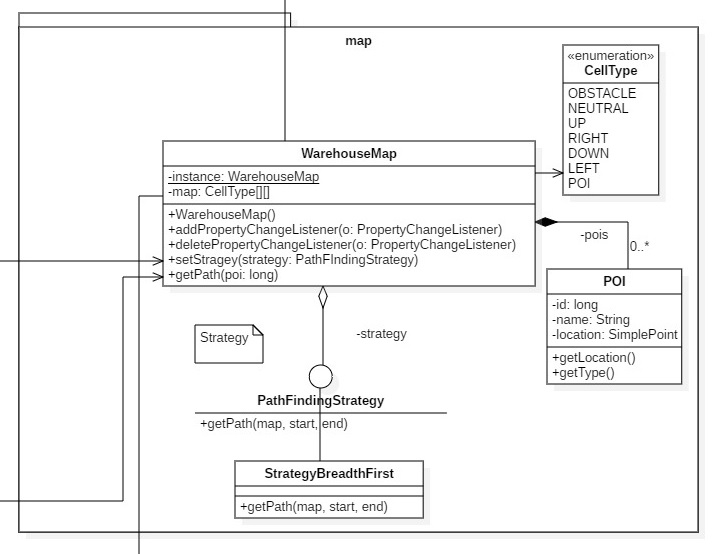
\includegraphics[scale=0.50]{res/diagrams/server/server_pack_map.jpg}
	\caption{Visione di dettaglio del package Map}
\end{figure}

\paragraph{Clients}
\subparagraph*{ }

\begin{figure}[H]
	\centering
	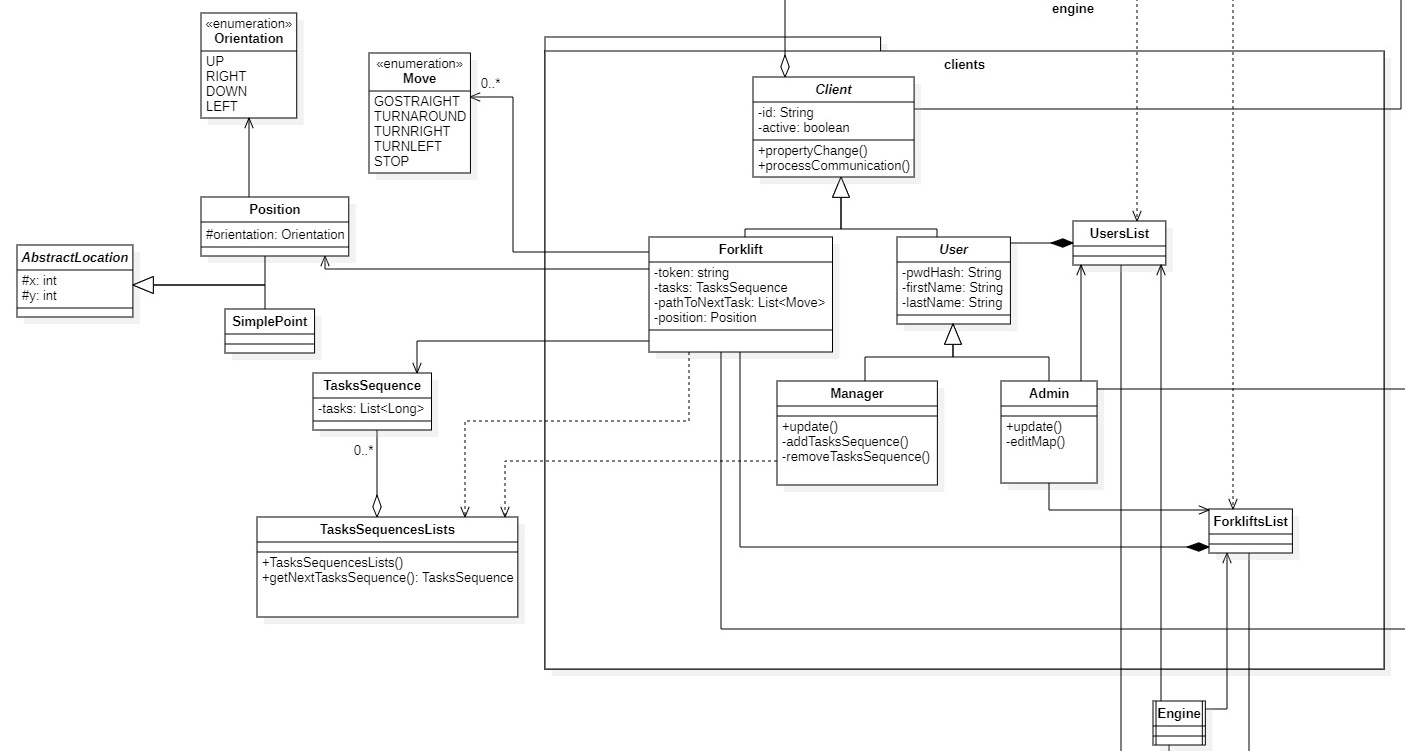
\includegraphics[scale=0.40]{res/diagrams/server/server_pack_clients.jpg}
	\caption{Visione di dettaglio del package Clients}
\end{figure}


\paragraph{Collisioni}
\subparagraph*{ }

\begin{figure}[H]
	\centering
	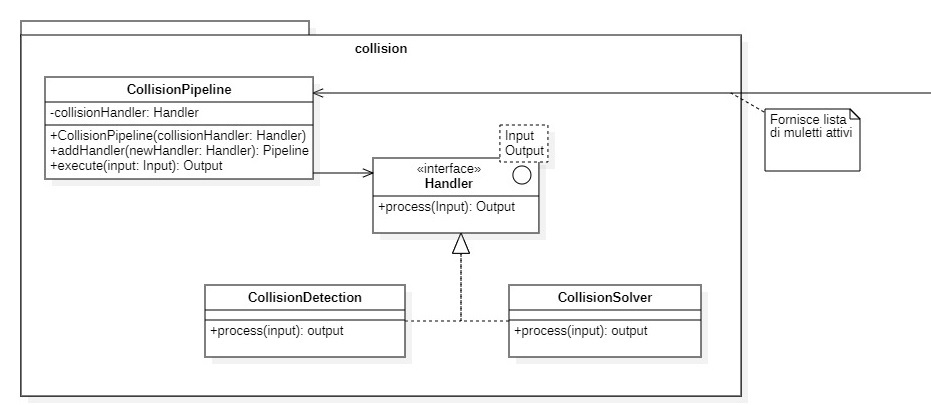
\includegraphics[scale=0.50]{res/diagrams/server/server_pack_collision.jpg}
	\caption{Visione di dettaglio del package Collision}
\end{figure}


\subsubsection{Persistence layer}

\begin{figure}[H]
	\centering
	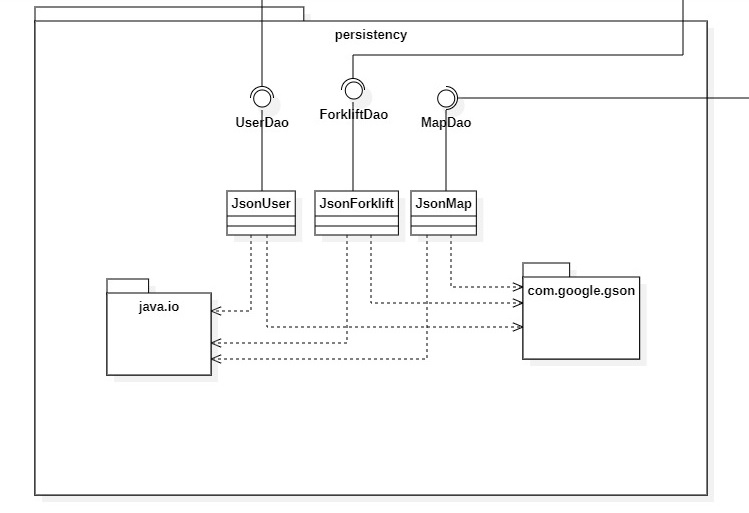
\includegraphics[scale=0.50]{res/diagrams/server/server_persistency.jpg}
	\caption{Visione di dettaglio del Persistence Layer}
\end{figure}
